% Options for packages loaded elsewhere
\PassOptionsToPackage{unicode}{hyperref}
\PassOptionsToPackage{hyphens}{url}
\PassOptionsToPackage{dvipsnames,svgnames,x11names}{xcolor}
%
\documentclass[
  letterpaper,
  DIV=11,
  numbers=noendperiod]{scrartcl}

\usepackage{amsmath,amssymb}
\usepackage{iftex}
\ifPDFTeX
  \usepackage[T1]{fontenc}
  \usepackage[utf8]{inputenc}
  \usepackage{textcomp} % provide euro and other symbols
\else % if luatex or xetex
  \usepackage{unicode-math}
  \defaultfontfeatures{Scale=MatchLowercase}
  \defaultfontfeatures[\rmfamily]{Ligatures=TeX,Scale=1}
\fi
\usepackage{lmodern}
\ifPDFTeX\else  
    % xetex/luatex font selection
\fi
% Use upquote if available, for straight quotes in verbatim environments
\IfFileExists{upquote.sty}{\usepackage{upquote}}{}
\IfFileExists{microtype.sty}{% use microtype if available
  \usepackage[]{microtype}
  \UseMicrotypeSet[protrusion]{basicmath} % disable protrusion for tt fonts
}{}
\makeatletter
\@ifundefined{KOMAClassName}{% if non-KOMA class
  \IfFileExists{parskip.sty}{%
    \usepackage{parskip}
  }{% else
    \setlength{\parindent}{0pt}
    \setlength{\parskip}{6pt plus 2pt minus 1pt}}
}{% if KOMA class
  \KOMAoptions{parskip=half}}
\makeatother
\usepackage{xcolor}
\setlength{\emergencystretch}{3em} % prevent overfull lines
\setcounter{secnumdepth}{-\maxdimen} % remove section numbering
% Make \paragraph and \subparagraph free-standing
\makeatletter
\ifx\paragraph\undefined\else
  \let\oldparagraph\paragraph
  \renewcommand{\paragraph}{
    \@ifstar
      \xxxParagraphStar
      \xxxParagraphNoStar
  }
  \newcommand{\xxxParagraphStar}[1]{\oldparagraph*{#1}\mbox{}}
  \newcommand{\xxxParagraphNoStar}[1]{\oldparagraph{#1}\mbox{}}
\fi
\ifx\subparagraph\undefined\else
  \let\oldsubparagraph\subparagraph
  \renewcommand{\subparagraph}{
    \@ifstar
      \xxxSubParagraphStar
      \xxxSubParagraphNoStar
  }
  \newcommand{\xxxSubParagraphStar}[1]{\oldsubparagraph*{#1}\mbox{}}
  \newcommand{\xxxSubParagraphNoStar}[1]{\oldsubparagraph{#1}\mbox{}}
\fi
\makeatother


\providecommand{\tightlist}{%
  \setlength{\itemsep}{0pt}\setlength{\parskip}{0pt}}\usepackage{longtable,booktabs,array}
\usepackage{calc} % for calculating minipage widths
% Correct order of tables after \paragraph or \subparagraph
\usepackage{etoolbox}
\makeatletter
\patchcmd\longtable{\par}{\if@noskipsec\mbox{}\fi\par}{}{}
\makeatother
% Allow footnotes in longtable head/foot
\IfFileExists{footnotehyper.sty}{\usepackage{footnotehyper}}{\usepackage{footnote}}
\makesavenoteenv{longtable}
\usepackage{graphicx}
\makeatletter
\def\maxwidth{\ifdim\Gin@nat@width>\linewidth\linewidth\else\Gin@nat@width\fi}
\def\maxheight{\ifdim\Gin@nat@height>\textheight\textheight\else\Gin@nat@height\fi}
\makeatother
% Scale images if necessary, so that they will not overflow the page
% margins by default, and it is still possible to overwrite the defaults
% using explicit options in \includegraphics[width, height, ...]{}
\setkeys{Gin}{width=\maxwidth,height=\maxheight,keepaspectratio}
% Set default figure placement to htbp
\makeatletter
\def\fps@figure{htbp}
\makeatother

\KOMAoption{captions}{tableheading}
\makeatletter
\@ifpackageloaded{caption}{}{\usepackage{caption}}
\AtBeginDocument{%
\ifdefined\contentsname
  \renewcommand*\contentsname{Table of contents}
\else
  \newcommand\contentsname{Table of contents}
\fi
\ifdefined\listfigurename
  \renewcommand*\listfigurename{List of Figures}
\else
  \newcommand\listfigurename{List of Figures}
\fi
\ifdefined\listtablename
  \renewcommand*\listtablename{List of Tables}
\else
  \newcommand\listtablename{List of Tables}
\fi
\ifdefined\figurename
  \renewcommand*\figurename{Figure}
\else
  \newcommand\figurename{Figure}
\fi
\ifdefined\tablename
  \renewcommand*\tablename{Table}
\else
  \newcommand\tablename{Table}
\fi
}
\@ifpackageloaded{float}{}{\usepackage{float}}
\floatstyle{ruled}
\@ifundefined{c@chapter}{\newfloat{codelisting}{h}{lop}}{\newfloat{codelisting}{h}{lop}[chapter]}
\floatname{codelisting}{Listing}
\newcommand*\listoflistings{\listof{codelisting}{List of Listings}}
\makeatother
\makeatletter
\makeatother
\makeatletter
\@ifpackageloaded{caption}{}{\usepackage{caption}}
\@ifpackageloaded{subcaption}{}{\usepackage{subcaption}}
\makeatother

\ifLuaTeX
  \usepackage{selnolig}  % disable illegal ligatures
\fi
\usepackage{bookmark}

\IfFileExists{xurl.sty}{\usepackage{xurl}}{} % add URL line breaks if available
\urlstyle{same} % disable monospaced font for URLs
\hypersetup{
  pdftitle={Toronto Transit Commission (TTC) Bus Delay},
  pdfauthor={Agam Sanghera, Ashita Diwan, Cheng Zhang, Yichun Liu},
  colorlinks=true,
  linkcolor={blue},
  filecolor={Maroon},
  citecolor={Blue},
  urlcolor={Blue},
  pdfcreator={LaTeX via pandoc}}


\title{Toronto Transit Commission (TTC) Bus Delay}
\usepackage{etoolbox}
\makeatletter
\providecommand{\subtitle}[1]{% add subtitle to \maketitle
  \apptocmd{\@title}{\par {\large #1 \par}}{}{}
}
\makeatother
\subtitle{Group 4}
\author{Agam Sanghera, Ashita Diwan, Cheng Zhang, Yichun Liu}
\date{}

\begin{document}
\maketitle


\subsection{Introduction}\label{introduction}

\begin{figure}[H]

{\centering \includegraphics{images/ttc_bus_crowded.avif}

}

\caption{Source: Toronto Star}

\end{figure}%

\subsection{Introduction}\label{introduction-1}

\begin{figure}[H]

{\centering 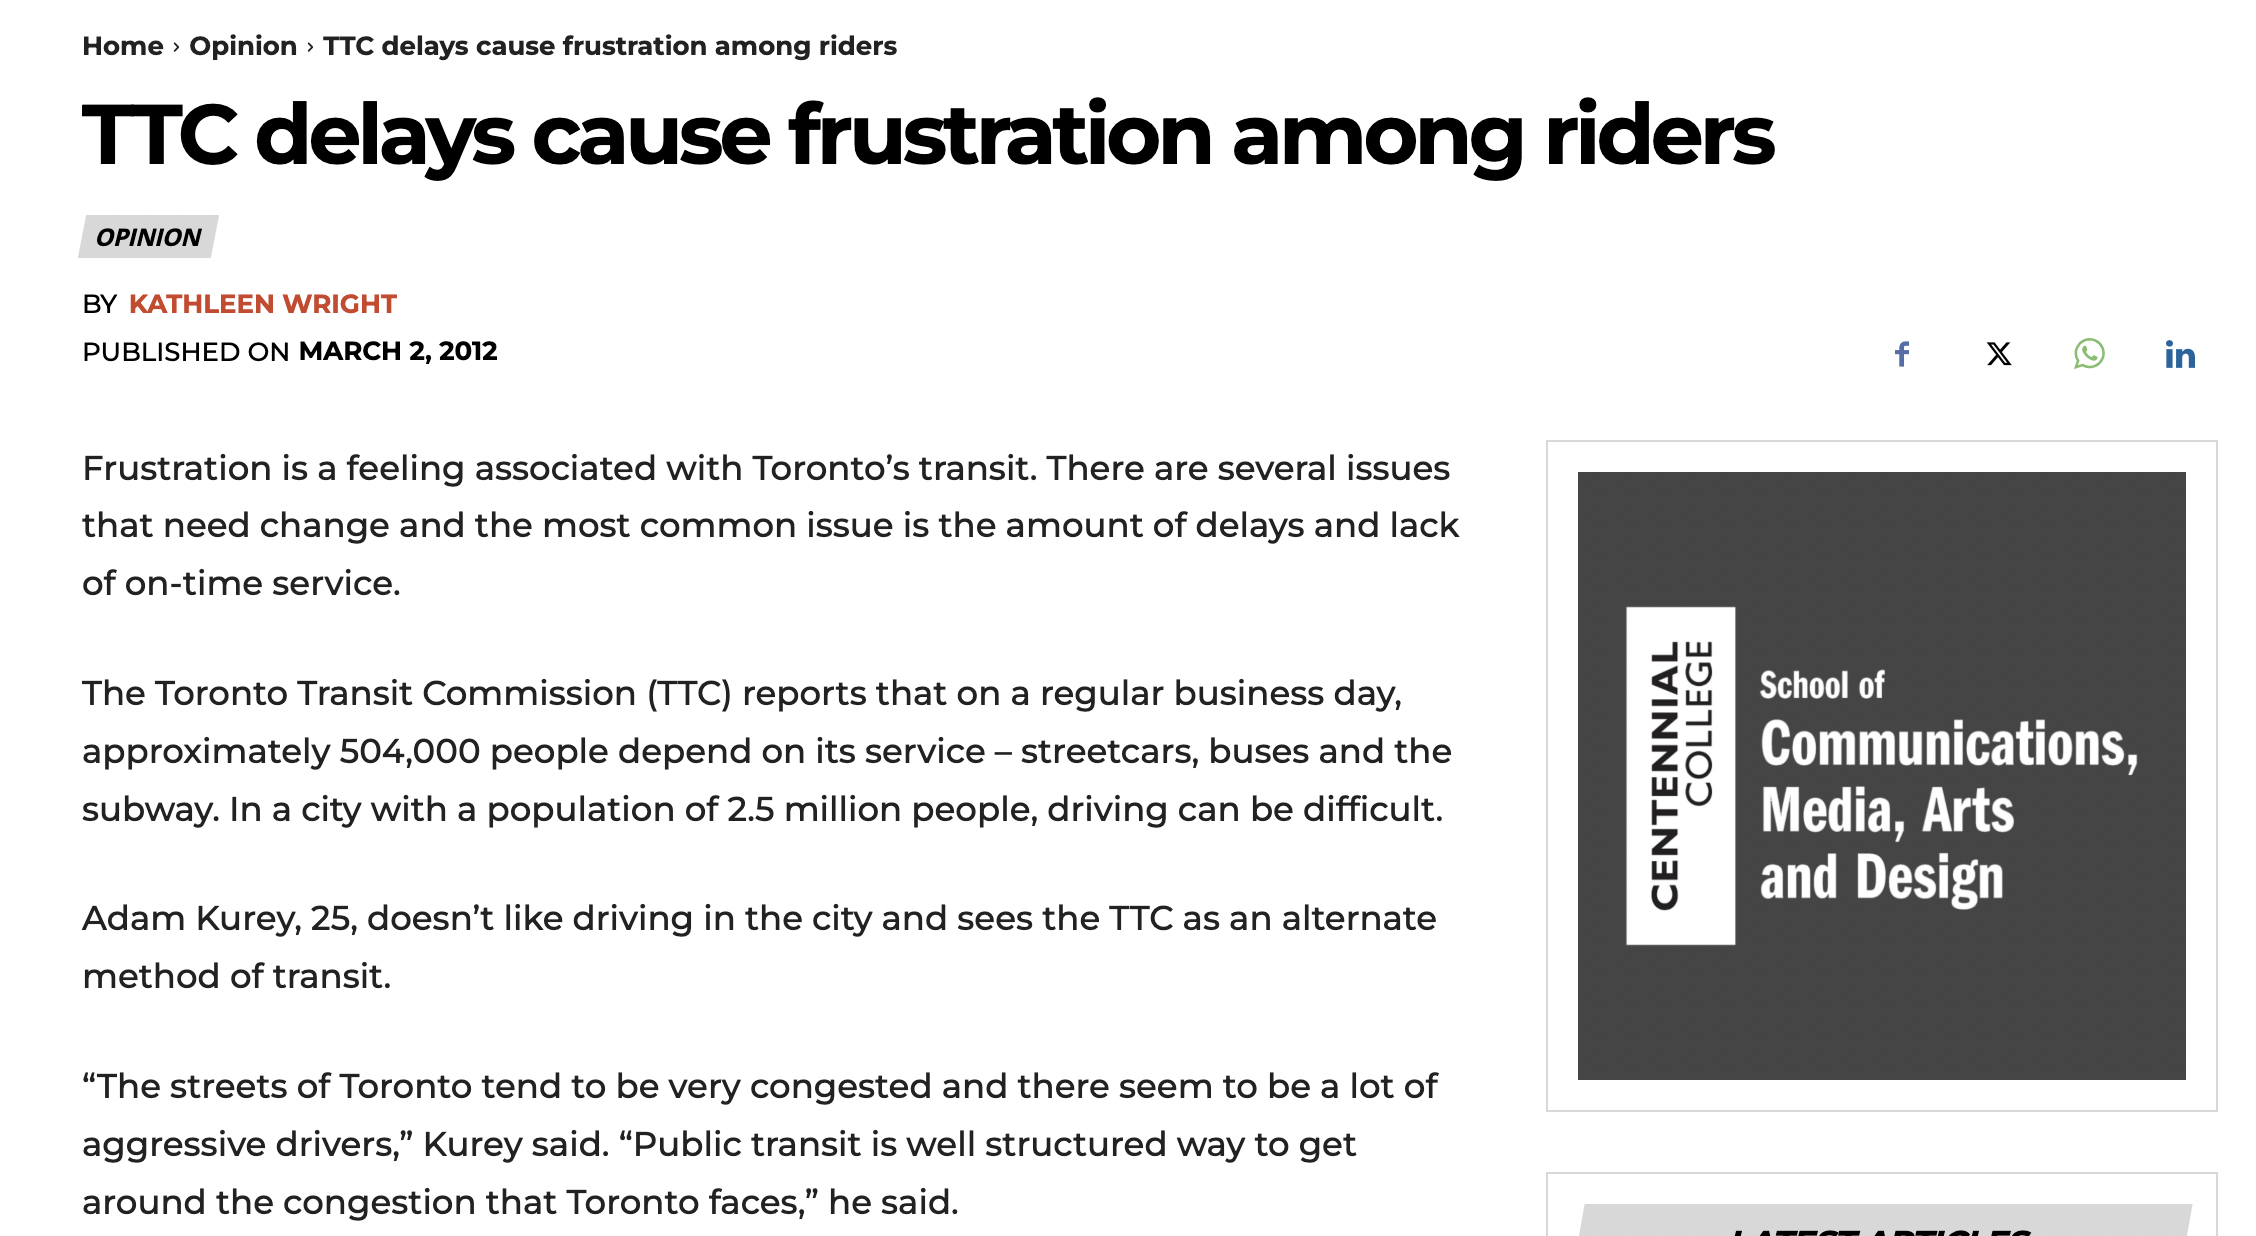
\includegraphics{images/ttc_bus_delay.png}

}

\caption{Source: Toronto Observer}

\end{figure}%

\subsection{Introduction}\label{introduction-2}

\begin{itemize}
\tightlist
\item
  Importance of the topic

  \begin{itemize}
  \tightlist
  \item
    Impacts on commuters
  \item
    Effects on transportation network
  \end{itemize}
\end{itemize}

\subsection{Introduction}\label{introduction-3}

\begin{itemize}
\tightlist
\item
  Purpose of the report

  \begin{itemize}
  \tightlist
  \item
    To analyze bus delays in the TTC system
  \item
    To identify key patterns, causes, and potential solutions for these
    delays
  \end{itemize}
\end{itemize}

\subsection{Introduction}\label{introduction-4}

\begin{itemize}
\tightlist
\item
  End product: build a logistic regression model to predict future bus
  delay duration

  \begin{itemize}
  \tightlist
  \item
    Better allocate resources
  \item
    Enhance bus service precision
  \end{itemize}
\end{itemize}

\section{Analysis}\label{analysis}

\subsection{Analysis}\label{analysis-1}

\begin{enumerate}
\def\labelenumi{\arabic{enumi}.}
\tightlist
\item
  \textbf{Loading and Preprocessing Data}
\item
  \textbf{Visualization}
\item
  \textbf{Modelling}
\end{enumerate}

\subsection{Analysis: Loading and Preprocessing
Data}\label{analysis-loading-and-preprocessing-data}

\begin{itemize}
\tightlist
\item
  Handle missing values,
\item
  Convert timestamp data to day parts, and
\item
  Clean data fields irrelevant to the analysis
\end{itemize}

\subsection{Analysis: Visualization}\label{analysis-visualization}

\begin{itemize}
\tightlist
\item
  Analyze distribution of delays,
\item
  Identify top routes and locations with frequent delay incidents, and
\item
  Visualize delays based on day and incident type
\end{itemize}

\subsection{Analysis: Modelling}\label{analysis-modelling}

\begin{itemize}
\tightlist
\item
  Logistic Regression model to predict

  \begin{itemize}
  \tightlist
  \item
    ``Short'', ``Medium'' or ``Long'' duration
  \end{itemize}
\item
  Cross-validation and randomized grid for hyperparameter tuning
\end{itemize}

\section{Results and Conclusions}\label{results-and-conclusions}

\subsection{Results}\label{results}

\begin{itemize}
\tightlist
\item
  \textbf{EDA}
\item
  \textbf{Model}
\end{itemize}

\subsection{EDA}\label{eda}

\begin{itemize}
\tightlist
\item
  \textbf{Distributions}
\item
  \textbf{Reclassified Labels}
\end{itemize}

\subsection{Model}\label{model}

\begin{itemize}
\tightlist
\item
  \textbf{Model Scores}
\item
  \textbf{Hyperparameter Tuning}
\item
  \textbf{Cross Validation}
\end{itemize}

\subsection{Conclusion}\label{conclusion}

\begin{itemize}
\tightlist
\item
  \textbf{Interpretation}
\item
  \textbf{Future Scope}
\end{itemize}

\subsection{Interpretation}\label{interpretation}

\begin{itemize}
\tightlist
\item
  \textbf{Comparison of Actual vs Prediction}
\item
  \textbf{Exlpanation of Results}
\end{itemize}

\subsection{Future Scope}\label{future-scope}

\begin{itemize}
\tightlist
\item
  \textbf{Improve Prediction of Long Delays}
\item
  \textbf{Experiment with other techniques}
\end{itemize}

\section{Thank you for your
attention}\label{thank-you-for-your-attention}




\end{document}
